\documentclass[11pt,a4paper]{article}
\usepackage[margin=24mm]{geometry}
\usepackage[T1]{fontenc}
\usepackage{lmodern,amsmath,amssymb,booktabs,longtable,array,hyperref,tikz}
\usetikzlibrary{arrows.meta,positioning,shapes.gates.logic.US,calc}
\hypersetup{hidelinks,pdfauthor={Quartz-4b7e},pdftitle={Student reference report}}
\setlength{\parindent}{0pt}\setlength{\parskip}{6pt}
\newcommand{\sa}[2]{#1/\mathrm{#2}}
\title{VLSI Testing: Homework 2\\Student reference report}
\author{Quartz-4b7e}\date{}
\begin{document}\maketitle
\textbf{Status.} This is an editable English reconstruction of the anonymized student report. It preserves the student's methods and reported conclusions. Independent verification notes appear at the end and distinguish confirmed results from errors. The original statement and anonymized report are included alongside this document.
\section{Fault detection and diagnosis with multiplexers}
\subsection{Two-input multiplexer}
The student's handwritten table follows the schematic: $x_i=0$ selects $g_0$ and $x_i=1$ selects $g_1$. Thus $f=\overline{x_i}g_0+x_i g_1$. The opening prose of the statement uses different input labels; this reconstruction explicitly follows the drawing and student's table.

The following table reconstructs the complete fault simulation. A heading $u/b$ means that line $u$ is stuck at $b$.
\begin{center}\small
\begin{tabular}{ccc|c|cccccccc}\toprule
$g_0$&$g_1$&$x_i$&Good&$g_0/0$&$g_0/1$&$g_1/0$&$g_1/1$&$x_i/0$&$x_i/1$&$f/0$&$f/1$\\\midrule
0&0&0&0&0&1&0&0&0&0&0&1\\
0&1&0&0&0&1&0&0&0&1&0&1\\
1&0&0&1&0&1&1&1&1&0&0&1\\
1&1&0&1&0&1&1&1&1&1&0&1\\
0&0&1&0&0&0&0&1&0&0&0&1\\
0&1&1&1&1&1&0&1&0&1&0&1\\
1&0&1&0&0&0&0&1&1&0&0&1\\
1&1&1&1&1&1&0&1&1&1&0&1\\\bottomrule
\end{tabular}\end{center}
The reported complete test set in $(g_0,g_1,x_i)$ order is
\[T=\{010,100,011,101\}.\]
Each stuck-at fault in the table changes the output for at least one of these vectors.

\subsection{Four-input multiplexer}
The first multiplexer produces $g_0$ from $h_0,h_1$, and the second produces $g_1$ from $h_2,h_3$. Select $x_i$ controls the first stage and $x_j$ controls the final stage. The student's diagnostic cubes use $X$ for a don't-care input.
\begin{center}
\begin{tabular}{cccccc|c|l}\toprule
$h_0$&$h_1$&$h_2$&$h_3$&$x_i$&$x_j$&Good $f$&Target\\\midrule
0&X&X&X&0&0&0&$g_0/1$\\
X&0&X&X&1&0&0&$g_0/1$\\
X&X&0&X&0&1&0&$g_1/1$\\
X&X&X&0&1&1&0&$g_1/1$\\
1&X&X&X&0&0&1&$g_0/0$\\
X&1&X&X&1&0&1&$g_0/0$\\
X&X&1&X&0&1&1&$g_1/0$\\
X&X&X&1&1&1&1&$g_1/0$\\\bottomrule
\end{tabular}\end{center}
Selecting the first branch isolates a fault on $g_0$ from one on $g_1$, and vice versa. A zero activates stuck-at-one; a one activates stuck-at-zero. Either of the two cubes for a target fault may be used.

\section{Deductive fault simulation}
The student's node names and circuit equations are
\[G=\overline{C+D},\quad I=BG,\quad H=\overline E,\quad J=I,\quad K=I,\quad L=\overline{A+J},\quad M=HK,\quad F=L+M.\]
Here $I$ is a fanout stem and $J,K$ are separately modeled branches.
\begin{center}
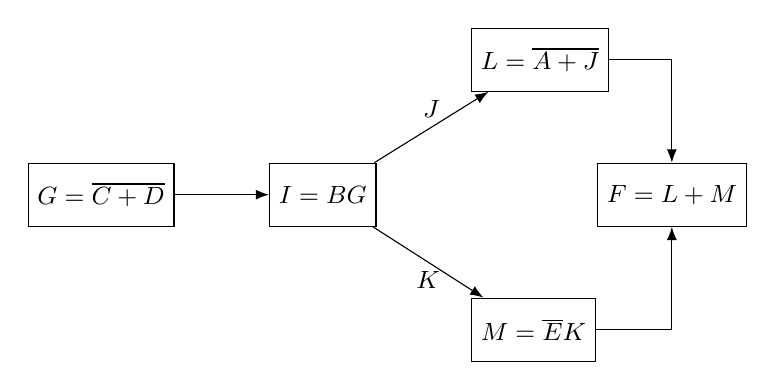
\begin{tikzpicture}[>=Latex,node distance=9mm and 12mm,b/.style={draw,minimum width=13mm,minimum height=8mm,font=\small}]
\node[b] (g) {$G=\overline{C+D}$};
\node[b,right=of g] (i) {$I=BG$};
\node[b,above right=of i] (l) {$L=\overline{A+J}$};
\node[b,below right=of i] (m) {$M=\overline E K$};
\node[b,right=28mm of i] (f) {$F=L+M$};
\draw[->] (g)--(i);\draw[->] (i)--node[above,font=\small]{$J$}(l);
\draw[->] (i)--node[below,font=\small]{$K$}(m);
\draw[->] (l)-|(f);\draw[->] (m)-|(f);
\end{tikzpicture}\end{center}
For input $ABCDE=01011$, the good values are $G=H=I=J=K=0$, $L=1$, $M=0$, and $F=1$. The handwritten propagation lists are
\begin{align*}
{\cal L}(G)&=\{D/0,G/1\},\\
{\cal L}(H)&=\{E/0,H/1\},\\
{\cal L}(I)&=\{D/0,G/1,I/1\},\\
{\cal L}(J)&=\{D/0,G/1,I/1,J/1\},\\
{\cal L}(K)&=\{D/0,G/1,I/1,K/1\},\\
{\cal L}(L)&=\{A/1,D/0,G/1,I/1,J/1,L/0\},\\
{\cal L}(M)&=\{M/1\},\\
{\cal L}(F)&=\{A/1,D/0,G/1,I/1,J/1,L/0,F/0\}.
\end{align*}
At $G$, input $D=1$ controls the NOR gate, so the inactive fault on $C$ does not propagate. At $I$, $G=0$ controls the AND gate, masking $B/0$. At $M$, both inputs are zero and no single upstream fault raises both; only $M/1$ raises its output. Finally, $L=1$ masks a change on $M$ at the output OR gate. The seven faults in ${\cal L}(F)$ are detected.

\section{Serial stuck-at fault simulation}
The submitted Verilog places a fault-injection multiplexer on each modeled line. Each two-bit control uses 0 for fault free, 1 for stuck at zero, 2 for stuck at one, and 3 for fault free. Thirteen modeled lines $A$ through $M$, including output $F$, give 26 single stuck-at faults.

The testbench initializes all controls to zero, then changes one control at a time through both stuck-at values. The four test vectors and reported detected sets are:
\begin{center}\begin{tabular}{cl}\toprule
Vector&Detected faults\\\midrule
10101&$A/0,F/1,L/1,M/1$\\
10010&$A/0,F/1,I/1,K/1,L/1,M/1$\\
00010&$A/1,F/0,J/1,L/0$\\
10100&$A/0,F/1,I/1,K/1,L/1,M/1$\\\bottomrule
\end{tabular}\end{center}
Their union is
\[\{A/0,A/1,F/0,F/1,I/1,J/1,K/1,L/0,L/1,M/1\},\]
so the reported coverage is $10/26=38.46\%$. These values describe the thirteen-line model explicitly implemented by the student. They make no claim about additional transistor or cell faults.

\section{Independent verification notes and source}
The detected sets can be checked by evaluating the Boolean equations once without a fault and once for every single forced line. The separate fault-free and faulty designs both declare module \texttt{circuit}; compile them separately. The original testbenches call FSDB dumping system tasks. The \texttt{MUX} case for control three is written \texttt{3'd3} despite the two-bit control; its numeric value remains three and the intended branch matches. Original source files remain unchanged.
\end{document}
